\chapter{Introduction} \label{chap:intro}
\renewcommand{\tabdir}{chapters/intro/tab}
\renewcommand{\figdir}{chapters/intro/fig}

This document is subdivided into three parts each of them adressing a different level of software hierarchy. The relation between the tree parts is depicted by an example in \figref{fig:engines_classes_processes}. 


Part \ref{part:modelEngines} contains a brief description of hydrological model engines implemented with the \software{echse} modeling framework. It provides information on the model engine's purpose and lists the important classes (\ie{} the types of objects that can be simulated) using references to the part \ref{part:classes}.

Part \ref{part:classes} holds a description of the classes, including information on state variables and external inputs, for example.

Part \ref{part:processes} addresses the mathematical representation of realworld hydrological processes, \ie{} the mechanisms  that cause the state variables to change their values over time. The concepts described in this part may be used by several of the classes portrayed in part \ref{part:classes}.


\begin{figure*}[htb]
  \centering
  \includegraphics[width=0.48\textwidth]{\figdir/engines_classes_processes.eps}
  \caption{Classes and processes as the basic building blocks of hydrological model engines. \label{fig:engines_classes_processes}}
\end{figure*}
